\documentclass[11pt]{article}

%Formatting Packages
\usepackage{graphicx}
\usepackage{float}
\usepackage[final]{pdfpages}
\usepackage[yyyymmdd]{datetime}
\renewcommand{\dateseparator}{--}
\usepackage{textcomp}
\usepackage[nottoc]{tocbibind}
\usepackage[english]{babel}
%\usepackage[top=0.9in, bottom=1in, left=1in, right=1in]{geometry} %Satan, but it helps you have more space

%Science packages
\usepackage{siunitx}
\usepackage{graphicx}
\usepackage[colorinlistoftodos]{todonotes}
\usepackage{hyperref}
\usepackage{url}
\usepackage[authoryear, sort]{natbib}
%\usepackage[style=authoryear]{biblatex}
%\addbibresource{\jobname-cites.bib}

% Custom commands
\newcommand*\chem[1]{\ensuremath{\mathrm{#1}}}
\title{Honors Thesis Proposal}
%\subtitle{Astrophysics PhD}
\author{Dylan Gatlin}
\date{\today}
\begin{document}
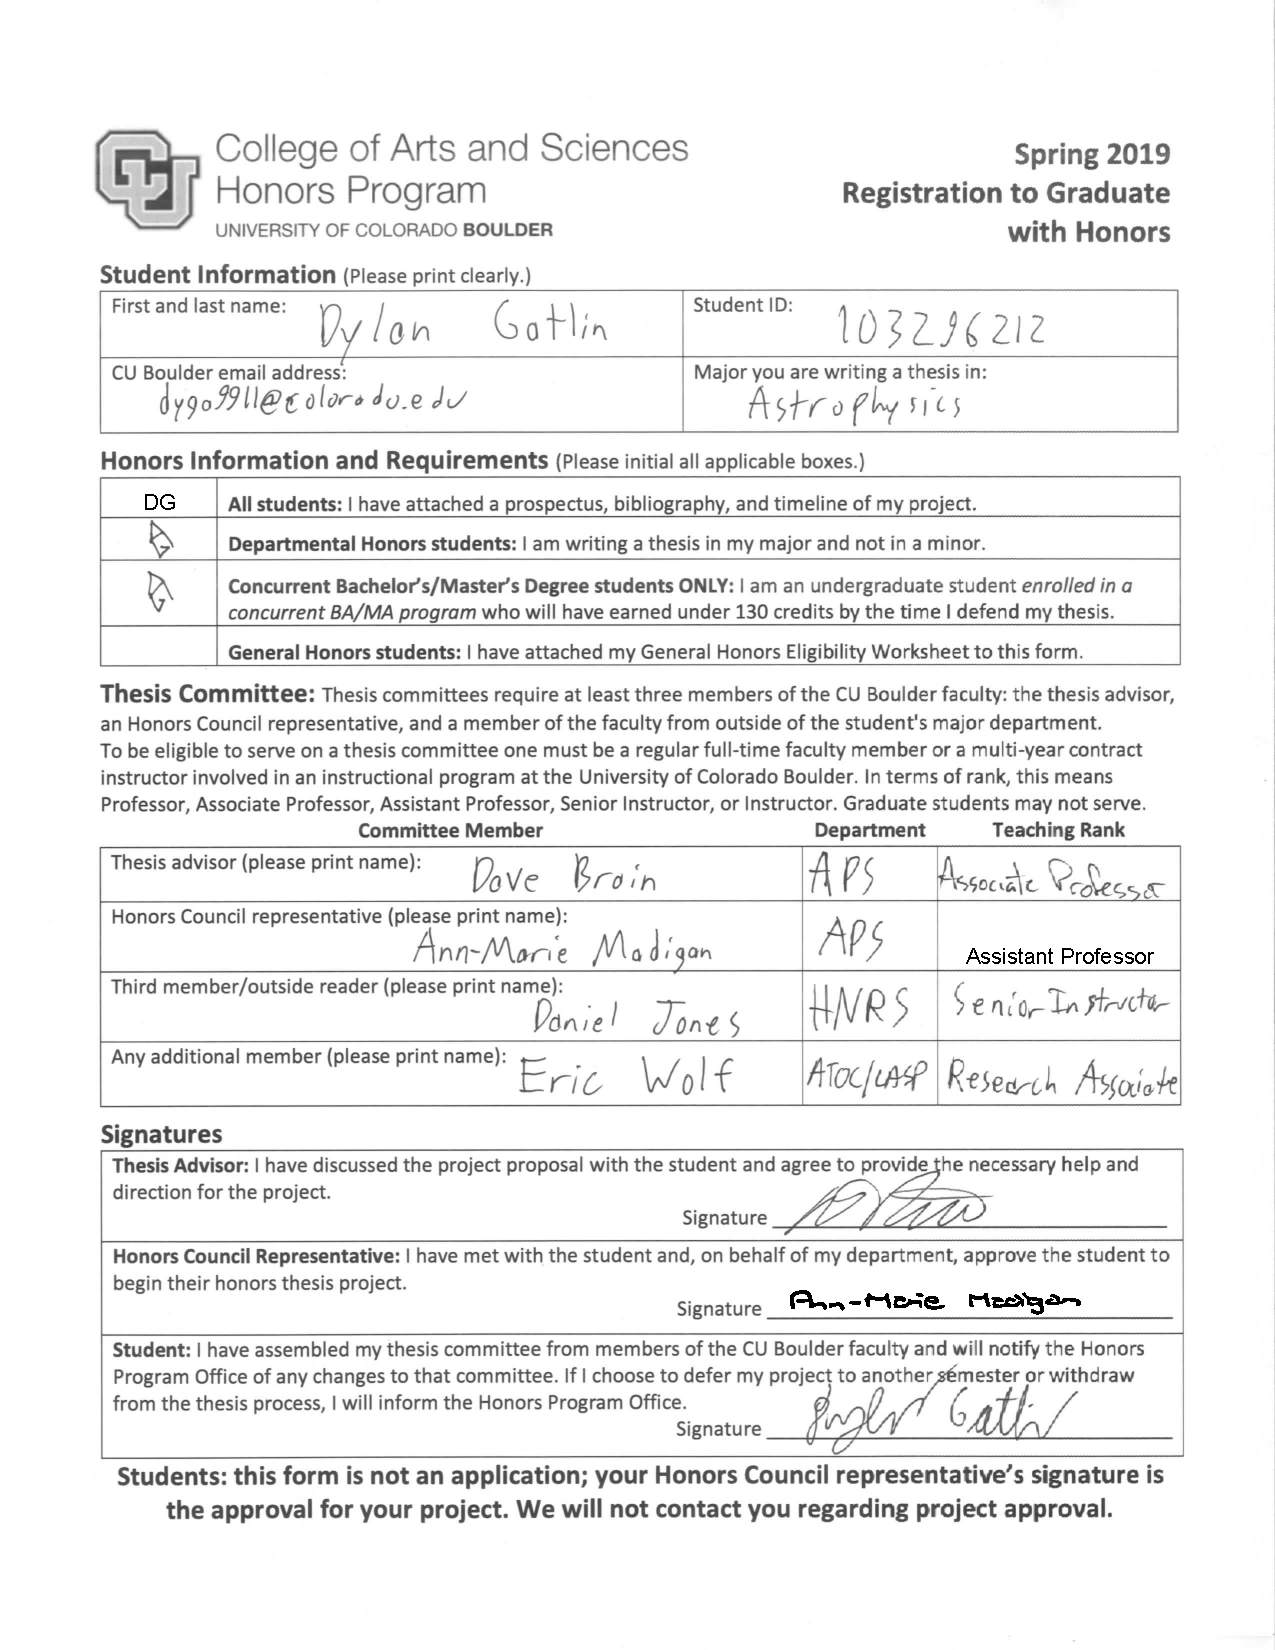
\includepdf{thesis_proposal_form.pdf}
\maketitle
\section*{Prospectus}
Exoplanetary astrophysics was a field that barely existed 20 years ago, and now it has become one of the most exciting fields in astrophysics. Until the Kepler mission, it was thought that exoplanets were rare, but we have since found there are about 100 billion exoplanets just in the Milky Way \citep{nexoplanets}. While most observed exoplanets are large gas giants close to their parent star, so called ``Hot Jupiters'', several terrestrial planets have also been found. Terrestrial exoplanets which receive similar solar insolation to that of Earth are the most likely candidates in the search for habitable worlds beyond Earth, and by extension, our most likely places to discover extraterrestrial life or a future home for humanity. To date, the list of exoplanets in the classical habitable zone is countably small, and not all of them are very close to Earth, but this will soon change with the recently launch of the Transiting Exoplanet Survey Satellite (TESS). TESS is expected discover thousands of exoplanets smaller than Neptune and dozens of Earth sized planets \citep{tesspredict}. In conjunction with the James Webb Space Telescope (JWST), we expect to have precise observations on a number of potentially habitable worlds in nearby star systems. However, it is known that exoplanets are likely to be tidally locked, as in they don't rotate relative to their star. This means they will have a substellar point, which always gets direct sunlight, a terminator, which gets a perpetual sunset, and an antistellar side, which never receives direct sunlight. Such an exotic world can't be compared to Earth, or any other object in the solar system. With such a new case for atmosphere parameters, the only way to characterize exoplanets is via coupled global circulation models (GCMs). These models have demonstrated that they are very different than what we would expect from the Earth, and our most Earth-like planet, TRAPPIST-1 d, is less likely to be habitable than TRAPPIST-1 e, a planet that receives only 60\% of the solar irradiance of Earth\citep{wolf17}.

Using GCMs for TRAPPIST-1 d, e, and f provided by Eric Wolf and the Planetary Spectrum Generator (PSG), a tool provided by NASA Goddard, I have created a data pipeline that can produce an exoplanet transit spectrum, simulating what telescopes like JWST will see during transits. In order to produce accurate spectra, an accurate GCM is essential. Simply assuming an exoplanet is ``Earth-like'' is unreasonable. Using this transit simulator, analysis can be done on the observable spectral features that JWST can detect, and signal to noise analysis will help the astrophysics community help prioritize their time on  JWST.

In addition to exoplanet spectra, GCMs can provide other windows into studying exoplanetary atmospheres. A GCM provides full global resolution of an exoplanet's surface, so in addition to a terminator atmosphere profile, Earth-facing atmosphere profiles can be made, which can be used to determine the change of the planet's thermal emission over the course of a year. So-called thermal phase curves measure the change in thermal brightness of a planet as it orbits its star, and can be variable in a way that could be detected with JWST. Thermal phase curves have the advantage of strong signal to noise due to large binning and long observation times. Using my pipeline, I can easily simulate thermal phase curves and use them to determine if there are clouds in the atmosphere and how those clouds are moving.

I will explore these two topics; transit spectra and thermal phase curves, in my honors thesis. Although the topics are slightly different branches of research, they're both competing techniques at analyzing exoplanets, and both will likely serve a major role in the coming years for JWST-era research. I anticipate my thesis will be broken into the following parts. In 1), I will explain the background of exoplanets, with an emphasis on the variables significant to thermal phase curves and transits. In 2), I will show Eric Wolf's climate models, and particularly focus on the terminator atmosphere profile and the global cloud patterns. I will compare fast rotators, which have smaller clouds formations, and slow rotators, which have large, permanent cloud patterns. In 3), I will explain the data pipeline I made and the PSG as a tool to simulate spectra. In 4), I will show transit spectra results, analyze their behavior, and identify and measure prominent features. In 5), I will do the equivalent analysis for thermal phase curves, and compare slow rotators versus fast rotators here. In 6), I will get into a noise analysis, and compare the reliability of the results of transits to that of thermal phase curves. Then I will conclude, stating the advantages of each.

\section*{Timeline}
In addition to the honors council, I will be submitting part of my honors thesis for the class PHYS 3050: Physics Writing. For this, I have a number of deadlines that will serve two purposes. Italicized dates will indicate that they are set by PHYS 3050.

\subsection*{{\it 2018-9-17}: Topic Brainstorm} Answer bullet-point questions about the project
\subsection*{{\it 2018-10-15}: First Draft} With an emphasis on the introduction and outline only
\subsection*{{\it 2018-10-31}: Second Draft} With an emphasis on completing sections 1-3
\subsection*{{\it 2018-10-29}: Third Draft} Completed and revised sections 1-3, with compiled plots and figures for part 4
\subsection*{{\it 2018-12-18}: Class Final} Completed sections 1-4, and a sufficient conclusion for it to be a complete paper worthy of submission, excluding thermal phase curves
\subsection*{2019-1-10: Research Completed} Using the time over winter break to finish any necessary research, write a first complete draft of the paper including all sections
\subsection*{2019-2-15: Second Complete Draft} Having completed the entire paper, continue the revision process
\subsection*{2019-3-15: Complete Final Draft} The final draft ready for submission to the review board
\subsection*{2019-3-25: Earliest Possible Defense} Subject to the approval of my board members
\subsection*{2019-4-8: Submit to Honors Program} Including defense copy, thesis copy, and title page
\bibliographystyle{abbrv}
\bibliography{proposal_citations}
\nocite{*}
\end{document}
